\documentclass[a4paper,14pt]{extarticle}
\usepackage[utf8]{inputenc}
\usepackage[T2A]{fontenc}
\usepackage[russian]{babel}
\usepackage{amssymb}
\usepackage{fancyvrb}
\usepackage[fleqn]{amsmath}
\usepackage{amsthm}
\usepackage{hyperref}
\usepackage{indentfirst}
\usepackage[left=3cm,right=1cm, top=2cm, bottom=2cm, bindingoffset=0cm]{geometry}
\hypersetup{
    colorlinks,
    citecolor=black,
    filecolor=black,
    linkcolor=black,
    urlcolor=black
}
% \textwidth = 16cm
% \usepackage{biblatex}
\usepackage{graphicx}
\usepackage{parskip}
% \addbibresource{bibliography.bib}
\newtheorem{theorem}{Теорема}
\newenvironment{rowequmat}[1]{\left(\array{@{}#1@{}}}{\endarray\right)}
\sloppy
\parindent=0.5cm
\title{Курсовой проект}
\author{\copyright Андрей Румянцев}
\date{29 ноября 2016}
\selectlanguage{russian}
\allowhyphens
\begin{document}
\begin{titlepage}
    \linespread{1.1}
    \begin{center}
    \fontsize{15pt}{15pt}\selectfont
    МИНИСТЕРСТВО ОБРАЗОВАНИЯ РЕСПУБЛИКИ БЕЛАРУСЬ\\
    \vspace{0.5cm}
    БЕЛОРУССКИЙ ГОСУДАРСТВЕННЫЙ УНИВЕРСИТЕТ\\
    \vspace{0.5cm}
    ФАКУЛЬТЕТ ПРИКЛАДНОЙ МАТЕМАТИКИ И ИНФОРМАТИКИ\\
    \vspace{0.5cm}
    \fontsize{13pt}{13pt}\selectfont
    \textit{КАФЕДРА МАТЕМАТИЧЕСКОГО МОДЕЛИРОВАНИЯ И АНАЛИЗА ДАННЫХ}\\
    \vspace{3.0cm}
    \fontsize{18pt}{18pt}\selectfont

    \vspace{0.5cm}
    \textbf{Статистическое оценивание параметров линейной регрессии с выбросами при наличии группирования наблюдений}\\
    \vspace{0.5cm}
    \fontsize{16pt}{16pt}\selectfont
    Курсовой проект\\
    \end{center}
    \vspace{3.5cm}
    \fontsize{14pt}{14pt}\selectfont
    \hspace{-0.25cm}
    \def\arraystretch{1.2}
    \begin{tabular}{l@{\hspace{3.25cm}}l}
    ~~~~~~~~~~~~~~~~~~~~~~~~~~~~~~~~~~~~~~~~~~  & Румянцева Андрея Кирилловича\\
    ~~~~~~~~~~~~~~~~~~~~~~~~~~~~~~~~~~~~~~~~~~  & студента 4 курса, специальность\\
    ~~~~~~~~~~~~~~~~~~~~~~~~~~~~~~~~~~~~~~~~~~  & "прикладная математика"\\
    ~~~~~~~~~~~~~~~~~~~~~~~~~~~~~~~~~~~~~~~~~~  & \\
    ~~~~~~~~~~~~~~~~~~~~~~~~~~~~~~~~~~~~~~~~~~  & Научный руководитель:\\
    ~~~~~~~~~~~~~~~~~~~~~~~~~~~~~~~~~~~~~~~~~~  & зав. кафедрой ММАД, \\
    ~~~~~~~~~~~~~~~~~~~~~~~~~~~~~~~~~~~~~~~~~~  &  канд. физ.-мат. наук, доцент\\
    ~~~~~~~~~~~~~~~~~~~~~~~~~~~~~~~~~~~~~~~~~~  &Бодягин Игорь Александрович\\
    
    
    \end{tabular}
    \vspace{4.5cm}
    \begin{center}
    \fontsize{16pt}{16pt}\selectfont
    Минск, 2018
    \end{center}
  \end{titlepage}

\newpage
\thispagestyle{empty}
\addtocounter{page}{-1}
\mbox{}
\newpage

\tableofcontents
\newpage
\begin{center}
    \section*{ВВЕДЕНИЕ}
\end{center}
\phantomsection
\addcontentsline{toc}{section}{ВВЕДЕНИЕ}
Существует несколько подходов для оценки параметров регрессии, но далеко не все устойчивы к возникновениям аномальных наблюдений, 
то есть таких наблюдений, которые не подчиняются общей модели. 
В реальной жизни аномальные наблюдения возникают постоянно. 
Такие наблюдения могут возникать по разным причинам: из-за ошибки измерения, из-за необычной природы входных данных.
По этой причине большинство методов просто неприменимо.
В прошлом веке в работах Хьюбера была заложена теория робастного оценивания.

Были предложены следующие робастные оценки\cite{Huber}:
\begin{itemize}
    \item М-Оценки
    \item R-Оценки
    \item L-Оценки
\end{itemize}
М-оценки -- некоторое подобие оценок максимального правдоподобия (ММП-оценки - частный случай), L-оценки строятся на основе линейных комбинаций порядковых статистик, R-оценки -- на основе ранговых статистик.

Будет предложен новый способ оценивания параметров регрессии,где используется группирование выборки, 
то есть такая модель наблюдений линейной  множественной  регрессии,  когда  вместо  истинных  значений
зависимой переменной наблюдаются номера классов (интервалов), в которые
попадают эти значения\cite{OLSforGrouping}. На практике были полностью реализованы описанные оценки и был произведен анализ оценок. 


\newpage
\section{Модель функции регрессии с аномальными наблюдениями и оценки ее параметров} \label{sec_1}
\subsection{Матмодель линейной регрессии с выбросами при наличии группирования наблюдений}
Введем модель линейной регрессию:\hfill\break
\begin{equation}
\begin{array}{c}
    \label{eq1}y_i=\beta_0+\beta_1 x_{i1}+\beta_2 x_{i2}+\dots+\beta_n x_{in}+\varepsilon_i, i=\overline{1,N},\\
    y_i= f(x_i,\beta)+\varepsilon_i,\\
    f(x_i,\beta)=\beta_0+\beta_1 x_{i1}+\beta_2 x_{i2}+\dots+\beta_n x_{in}
\end{array}
\end{equation}
или, в векторной форме:
\begin{eqnarray}
    \label{eq2}y_i= 
    \begin{pmatrix}
        \beta_0\\
        \beta_1\\
        \dots\\
        \beta_n
    \end{pmatrix}\times
    \begin{pmatrix}
        1\\
        x_{i1}\\
        \dots\\
        x_{in}
    \end{pmatrix}^{T}+ \varepsilon_i,
\end{eqnarray}
где $y_i$ -- $i$-е наблюдение из $N$ наблюдений($N$-объем выборки), $x_i=(x_{i1},x_{i2},\dots,x_{in})$ регрессоры, \{$\beta_k, k=\overline{0,n}$\}-- параметры регрессии, а $\varepsilon_i$ -- случайная ошибка $i$-го эксперемента, распределение которой подчиняется нормальному закону с нулевым математическим ожиданием и дисперсией $\sigma^2$.

Пусть вместо истинных значений $y_i$, заданных формулами (\ref{eq1})-(\ref{eq2}), 
наблюдаются значения с искажениями, описываемыми соотношением:
\begin{eqnarray}
    \label{eq3}y_i^{\widetilde{\varepsilon}}=(\xi_i)y_i+ (1-\xi_i)\eta_i,
\end{eqnarray}
где $\xi_i$ принимает значение, равное 1, с вероятностью $1-\widetilde{\varepsilon}$ и значение, равное 0, с вероятностью $\widetilde{\varepsilon}$, т.е.:
\begin{eqnarray}\label{eq4}
    \begin{cases}
        p(\xi_i=0)=\widetilde{\varepsilon},\\
        p(\xi_i=1)=1-\widetilde{\varepsilon},
    \end{cases},
\end{eqnarray}
которая называется функцией линейной регрессии с выбросами. $\eta_i$-случайная величина из некоторого вообще говоря неизвестного распределения.
Параметр $\xi_i$ имеет следующий содержательный смысл: если $\xi_i=0$, то вместо истинного значения мы наблюдаем выброс, если $\xi_i=1$, то наблюдается истинное значение.
Переменную $\widetilde{\varepsilon}$ будем называть долей аномальных наблюдений. Величины $\xi_i, x_i$ и $\eta_i$ являются независимыми.

Каждый $y_i$ принадлежит нормальному распределению:
\begin{eqnarray}
    \label{eq12} y_i=f(x_i,\beta)+\varepsilon_i \sim \mathcal{N}(f(x_i,\beta),\sigma^2).
\end{eqnarray}

Разделим множество значений функции регрессии, т.е множество $\mathcal{R}$, на $k$ полуинтервалов:
\begin{eqnarray}
    \mathcal{R}=(-\infty,a_1]\bigcup(a_1,a_2]\bigcup \dots \bigcup(a_{k-1},+\infty ).
\end{eqnarray}
Обозначим полученные интервалы: $\nu_0,\dots,\nu_{k-1}$.

Далее в работе будем считать, что вместо истинных значений зависимых переменных $y_i$ наблюдается только номер класса, к которому это наблюдение попало.
Тогда для каждого $y_i$ будем наблюдать лишь номер полуинтервала $\mu_i$, в который он попал.
\begin{eqnarray}
    \mu_i=j, \textup{если $y_i$ отнесли к полуинтервалу $\nu_j$}.
\end{eqnarray}

В данной работе решается задача статистического оценивания параметров модели \{$\beta_k, k=\overline{0,n}$\} по известным группированным наблюдениям с аномалиями.




 \subsection{Метод наименьших квадратов}
Предлоположим, что случайные ошибки подчиняются нормальному закону распределения вероятностей:
\begin{eqnarray}
    \label{eq5}L\{\varepsilon_i\}=N_1(0,\sigma^2), i = \overline{1,n}.
\end{eqnarray}
Строим логарифмическую функцию правдоподобия. В силу (\ref{eq1}) и (\ref{eq2}) имеем:
\begin{eqnarray}
    L\{y_i\}=N_1(f(x_i;\beta), \sigma^2).
\end{eqnarray}
Логарифмическая функция правдоподобия выглядит так\cite{Kharin}:
\begin{eqnarray}
    l(\beta)=\ln \prod_{i=1}^{n}(\frac{1}{\sqrt{2\pi}\sigma}e^{-\frac{(y_i-f(x_i;\beta))^2}{2\sigma^2}})&=&-\frac{1}{2}n\ln{2\pi\sigma^2}-\frac{1}{2\sigma^2}R^2(\beta),\\
    R^2(\beta)=\sum_{i=1}^{n}(\delta y_i)^2&=&\sum_{i=1}^{n}(y_i-f(x_i,\beta))^2\geq 0.
\end{eqnarray}
Тогда оценка методом наименьших квадратов из формул (\ref{eq4}), (\ref{eq5}) такова:
\begin{eqnarray}
    \hat{\beta}=arg \min_{\beta}R^2(\beta).
\end{eqnarray}

\subsection{М-оценки}
Швейцарский статистик П.Хьюбер предложил использовать М-оценки \cite{Kharin}, которые являются решениями экстремальных задач вида:
\begin{eqnarray}
    \sum_{i=1}^{n}\phi(x_t;\beta)\rightarrow \min_{\beta},
\end{eqnarray}
где $\phi(\cdot;\beta)$-некоторая функция, определяющая конкретный тип оценок и их точность.

Очевидно, что $\phi(\cdot;\beta)\equiv - \ln{p(\cdot;\beta)}$ дает обычную оценку максимального правдоподобия, построенную по модели без выбросов (\ref{eq1}).

Рассмотрим теперь некоторые способы выбора функции $\phi(\cdot;\beta)$ для решения экстремальной задачи в M-оценках.

Для начала определим:
\begin{eqnarray}
    u_i=y_i^{\widetilde{\varepsilon}}-(\beta_0+\beta_1 x_{i1}+\beta_2 x_{i2}+\dots+\beta_n x_{in}).
\end{eqnarray}
Тогда существует такие методы\cite{RobustRegression}:\hfill\break
\begin{center}
\begin{tabular}{ |p{3cm}|p{10cm} | }
    \hline
    \multicolumn{2}{|c|}{Способы выбора $\phi(\cdot;\beta)$} \\
    \hline
    Метод& Целевая функция\\
    \hline
    Метод Наименьших Квадратов&$\phi(\cdot;\beta)_{OLS}=u^2$\\
    \hline
    Хьюбера&$\phi(\cdot;\beta)_{H}=
        \begin{cases}
            \frac{1}{2}u^2, |u|\leq k,\\
            k|u|-\frac{1}{2}k^2, |u|>k
        \end{cases}$\\
    \hline
    Биквадратный& $\phi(\cdot;\beta)_{B}=
    \begin{cases}
        \frac{k^2}{6}(1-[1-(\frac{u}{k})^2]^3), |u|\leq k\\
        \frac{k^2}{6}, |u|>k
    \end{cases}$\\
    \hline
\end{tabular}
\end{center}
\newpage

\section{Построение оценок параметров регресии с помощью группирования выборки}\label{sec4}
Будем работать с моделью регрессии (\ref{eq3}), предполагая что имеем регрессию без выбросов (\ref{eq1}). 

Введем обозначение для функции распределения стандартного нормального закона:
\begin{eqnarray}
    \Phi(x)=\frac{1}{\sqrt{2}\sigma}\int_{-\infty}^{x}e^{\frac{-t^2}{2}}dt.
\end{eqnarray}
Тогда функцию распределения нормального закона с параметрами $\mu,\sigma^2$ можно представить как:
\begin{eqnarray}
    F(x)=\Phi(\frac{x-\mu}{\sigma}),
\end{eqnarray}
где $\sigma = \sqrt{\sigma^2}$. \hfill\break
Обозначим:
\begin{eqnarray}
    \textup{erf}(x)=\frac{2}{\sqrt{\pi}}\int_0^{x}e^{-t^2}dt.
\end{eqnarray}
Тогда:
\begin{eqnarray}
    \Phi(x)= \frac{1}{2} \Big[1+\textup{erf}\Big(\frac{x}{\sqrt{2}} \Big) \Big].
\end{eqnarray}
Поэтому:
\begin{eqnarray}
    F(x)= \frac{1}{2} \Big[1+\textup{erf}\Big(\frac{x-\mu}{\sqrt{2}\sigma} \Big) \Big].
\end{eqnarray}
При модельных предположениях (\ref{eq12}) вероятность попадания $y_i$ в полуинтервал $\nu_j$ равна:
\begin{multline}
    P\{y_i\in\nu_j\}= F_{y_i}(a_{j+1})-F_{y_i}(a_{j})=\\
    =\begin{cases}
        \frac{1}{2}(\textup{erf}(\frac{a_{j+1}-f(x_i,\beta)}{\sqrt{2}\sigma})-\textup{erf}(\frac{a_{j}-f(x_i,\beta)}{\sqrt{2}\sigma})),~j=\overline{1,k-2}\\
        \frac{1}{2}(1+\textup{erf}(\frac{a_{1}-f(x_i,\beta)}{\sqrt{2}\sigma})),~j=0\\
        \frac{1}{2}(1+\textup{erf}(\frac{a_{k-1}-f(x_i,\beta)}{\sqrt{2}\sigma})),~j=k-1
    \end{cases}.
\end{multline}
Понятно, что:
\begin{eqnarray}
    P(\mu_i=j)=P(y_i\in \nu_{\mu_i}).
\end{eqnarray}



\subsection{Построение функции правдоподобия}\label{sec4_1}
Составим функцию правдоподобия:
\begin{eqnarray}
    \label{eq22}l(\beta,\sigma^2, \nu_0,\dots, \nu_{k-1})&=&\textup{ln}(\prod_{i=1}^{n}P(\mu_i=j))=\\
    \label{eq23}&=&\sum_{i=1}^{n}\ln(P(\mu_i=j)).
\end{eqnarray}
Известно приближение для функции $\textup{erf}(x)$:
\begin{eqnarray}
    \label{eq24}(\textup{erf} x)^2&\approx& 1- \exp(-x^2 \frac{\frac{4}{\pi}+ax^2}{1+ax^2}),\\
    \nonumber a&=&\frac{8}{3\pi}\frac{3-\pi}{\pi -4}.
\end{eqnarray}
Оно считается достаточно точным для $x$ близких к $0$ и к $\infty$ \cite{Winitzki}. \hfill\break
Найдем производную для этого приближения:
\begin{eqnarray}
    \label{eq26}\textup{erf}'(x) = \exp(-x^2 \frac{\frac{4}{\pi}+ax^2}{1+ax^2}) \frac{-2x\frac{\frac{4}{\pi}+ax^2}{1+ax^2}+(2ax^3)\frac{\frac{4}{\pi}+ax^2}{1+ax^2}-\frac{2ax^3}{1+ax^2}}{2\sqrt{1- \exp(-x^2 \frac{\frac{4}{\pi}+ax^2}{1+ax^2})}}.
\end{eqnarray}
Будем максимизировать функцию $l$.
Для этого будем искать нули ее производной. Вычисление будем производить с помощью вычислительных методов (будем использовать метод секущих), так как из-за сложного
вида производной вычислить ее аналитически не представляется возможным.
\begin{multline}
    \label{eq27}\frac{\delta l}{\delta \beta}=\frac{\delta \sum_{i=1}^{n}\ln(P(\mu_i=j))}{\delta \beta}=\frac{\delta \sum_{i=1}^{n}\ln P(y_i\in \nu_{\mu_i})}{\delta \beta}=~\\
    =\frac{\delta \sum_{i=1}^{n} \ln(\frac{1}{2}(\textup{erf}(\frac{a_{\mu_i+1}-f(x_i,\beta)}{\sqrt{2}\sigma})-\textup{erf}(\frac{a_{\mu_i}-f(x_i,\beta)}{\sqrt{2}\sigma})) )         }{\delta \beta}=~\\
    =  \sum_{i=1}^{n}\Big((1-(\delta_{\mu_i 0}+\delta_{\mu_i k-1}))\frac{(\textup{erf'}(\frac{a_{\mu_i+1}-f(x_i,\beta)}{\sqrt{2}\sigma})-\textup{erf'}(\frac{a_{\mu_i}-f(x_i,\beta)}{\sqrt{2}\sigma}))}{ (\textup{erf}(\frac{a_{\mu_i+1}-f(x_i,\beta)}{\sqrt{2}\sigma})-\textup{erf}(\frac{a_{\mu_i}-f(x_i,\beta)}{\sqrt{2}\sigma}))}+~\\
    +(\delta_{\mu_i 0}+\delta_{\mu_i k-1})\frac{\textup{erf'}(\frac{a_{\mu_i}-f(x_i,\beta)}{\sqrt{2}\sigma})}{(1+\textup{erf}(\frac{a_{\mu_i}-f(x_i,\beta)}{\sqrt{2}\sigma}))}\Big)  (-1) \frac{\delta f(x_i,\beta)}{\delta \beta} )=~
\end{multline}
\begin{multline}
    \nonumber 
    =-\sum_{i=1}^{n}\begin{pmatrix}
        1\\
        x_{i1}\\
        \dots\\
        x_{in}
    \end{pmatrix}\times  \Big((1-(\delta_{\mu_i 0}+\delta_{\mu_i k-1}))\frac{(\textup{erf'}(\frac{a_{\mu_i+1}-f(x_i,\beta)}{\sqrt{2}\sigma})-\textup{erf'}(\frac{a_{\mu_i}-f(x_i,\beta)}{\sqrt{2}\sigma}))}{ (\textup{erf}(\frac{a_{\mu_i+1}-f(x_i,\beta)}{\sqrt{2}\sigma})-\textup{erf}(\frac{a_{\mu_i}-f(x_i,\beta)}{\sqrt{2}\sigma}))}+~\\
    +(\delta_{\mu_i 0}+\delta_{\mu_i k-1})\frac{\textup{erf'}(\frac{a_{\mu_i}-f(x_i,\beta)}{\sqrt{2}\sigma})}{(1+\textup{erf}(\frac{a_{\mu_i}-f(x_i,\beta)}{\sqrt{2}\sigma}))}\Big)  ,~
\end{multline}
где $\delta_{ij}$ - символ Кронекера.

Доказано, что максимизируя функцию правдоподобия (\ref{eq22}), можем получить состоятельную оценку\cite{OLSforGrouping} параметров.

Итак, выражение (\ref{eq27}) и будем использовать для метода секущих, приближая $\textup{erf}'(x)$ с помощью выражения (\ref{eq26}).

\subsection{Метод секущих}\label{sec4_2}
Так как мы не можем привести систему $ \frac{\delta l}{\delta \beta}=0$ к виду, удобному для итерации, то нам придется искать ее нули с помощью метода секущих.
Введем вектор ошибки $\check{\varepsilon}^{(k)}=\beta^{*}-\beta^{(k)}$. Тогда для его определения имеем:
\begin{eqnarray}
    \frac{\delta l (\beta^{(k)}+\check{\varepsilon}^{(k)})}{\delta \beta}=0.
\end{eqnarray}
Строя разложение левой части по формуле Тейлора и ограничиваясь лишь линейными членами\cite{NumericalMethods}, будем иметь систему:
\begin{eqnarray}
    \frac{\delta }{\delta \beta}\frac{\delta l (\beta^{(k)}}{\delta \beta}\Delta \beta^{(k)}=-\frac{\delta l (\beta^{(k)})}{\delta \beta}.
\end{eqnarray}
Если матрица $\frac{\delta }{\delta \beta}\frac{\delta l (\beta^{(k)}}{\delta \beta}$ невырожденная (а в нашем случае она диагональная), то из этой системы можно единственным образом найти $\Delta \beta^{(k)}$ и построить приближение:
\begin{eqnarray}
    \beta^{(k+1)}=\beta^{(k)}+\Delta \beta^{(k)}.
\end{eqnarray}

Так как для второй производной $l$ получится довольно сложное выражение, то будем приближать ее с помощью выражения:
\begin{eqnarray}
    \frac{\delta }{\delta \beta_j}\frac{\delta l(\beta_1^{(k)},\dots, \beta_n^{(k)}) }{\delta \beta}\approx \frac{\frac{\delta l(\beta_1^{(k)},\dots,\beta_j^{(k)},\dots, \beta_n^{(k)}) (\beta^{(k)}}{\delta \beta}-\frac{\delta l(\beta_1^{(k)},\dots,\beta_j^{(k-1)},\dots, \beta_n^{(k)}) (\beta^{(k)}}{\delta \beta}}{\beta_j^{(k)}-\beta_j^{(k-1)}}.
\end{eqnarray}

Теперь имеем нули производной функции $l$, а также ее значения на границе отрезка $[a,b]$.
Переберем эти значения и таким образом найдем значение вектора $\hat{\beta}$, где она достигает своего максимального значения.
% \subsection{Оценка сходимости метода секущих}
% Так как метод секущих является частным случаем метода Ньютона, то приведем теоремы




\subsection{Переклассификация выборки}\label{sec4_3}
На данном этапе для каждого $x_i$ имеем класс $\mu_i$: т.е. пару $(x_i,\mu_i)$.
Теперь попытаемся переклассифицировать выборку. 
Для этом будем строить новую выборку такого же объема $N$.
Будем идти по каждому элементу $(x_i, \mu_i)$ выборки и для этого наблюдения построим новое:
\begin{eqnarray}
    (x_i, \check{\mu}_i),
\end{eqnarray}
где $\check{\mu}_i$ получен по методу $L$-средних.\hfill\break
\begin{eqnarray}
    \check{\mu}_i = \arg\max_j \sum_{k \in V_i,~k\neq i} \delta_{\check{\mu}_k j}~,
\end{eqnarray}
где $V_i$ множество индексов $l$ первых $L$ векторов $x_l$, отсортированных по возрастанию расстояния до вектора $x_i$.

Итак, переклассифицировав выборку, применим к ней функцию правдоподобия из уравнений (\ref{eq22}-\ref{eq23}), только используя теперь новые классы $\check{\mu}_i$ вместо $\mu_i$. 
Аналогично пунктам \ref{sec4_1}-\ref{sec4_2} максимизируем ее и найдем новую оценку параметров $\hat{\beta}$.

\newpage
\section{Реализация оценок на практике}
На практике построение оценок является нетривиальной задачей, так как метод секущих имеет свои недостатки.
Для метода секущих необходимо, чтобы корни уравнения были отделены, но не существует способа отделения корней в общем случае.
Поэтому для решения уравнения нам нужны дополнительные параметры:
\begin{itemize}
    \item границы отрезка, на котором находятся предполагаемая оценка $\hat{\beta}$;
    \item разность векторов двух начальных приближений $\hat{\beta}^{(1)} - \hat{\beta}^{(0)}$;
    \item шаг для каждой компоненты $\hat{\beta}_i^{(0)}$.
\end{itemize}
Тогда решая методом секущих уравнение
\begin{eqnarray}
    \frac{\delta l (\beta)}{\delta \beta}=0
\end{eqnarray}
на каждом из отрезков найдем возможные $\hat{\beta}$. Найдя среди полученных приближений $\hat{\beta}$ то, 
на котором функция правдоподобия (\ref{eq22}-\ref{eq23}) достигает максимума, 
найдем решение.



\subsection{Моделирование функции регрессии с аномальными наблюдениями}\label{sec3}
Для начала смоделируем функцию регрессии по методу (\ref{eq3}). Для удобства моделируем регрессию с одномерными регрессорами $x_i, i=\overline{1,N}$.\hfill\break
Воспользуемся такими параметрами:\hfill\break
\begin{center}
\begin{tabular}{|p{5cm}|p{5cm}|}
    \hline
    \multicolumn{2}{|c|}{Параметры программы} \\
    \hline
    Переменная&значение\\
    \hline
    Размер выборки $N$& 1000\\
    \hline
    Доля выбросов $\widetilde{\varepsilon}$& 0.1\\
    \hline
    Параметры регрессии $\beta$& $(100,4)$\\
    \hline
    Регрессоры $x_i$ & $\sim U(-5,5)$\\
    \hline
    $\varepsilon_i$&$\sim N(0,16)$\\
    \hline
    $\eta_i$&$\sim N(100,100)$\\
    \hline
\end{tabular},
\end{center}
$U(-5,5)$ - равномерное распределение на отрезке $[-5,5]$.\hfill\break
Получаем такой график:\hfill\break
\begin{figure}[ht!]
    \centering
    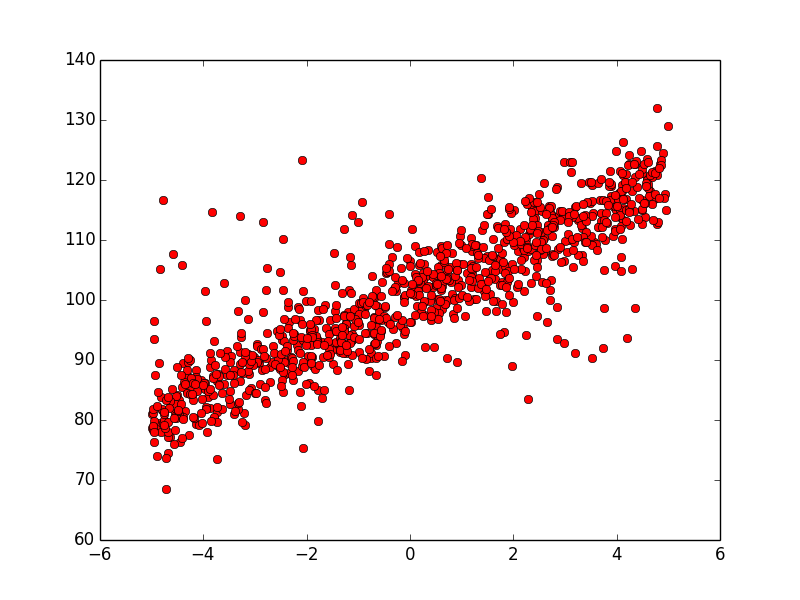
\includegraphics[width=100mm]{pics/graphic.png}
    \caption{Вывод графика рассеяния $(y_i,x_i)$\label{overflow}}
\end{figure}

\subsection{Компьютерные эксперименты с построенными оценками}
\begin{center}
    \begin{tabular}{|p{5cm}|p{5cm}|}
        \hline
        \multicolumn{2}{|c|}{Параметры программы} \\
        \hline
        Переменная&значение\\
        \hline
        Размер выборки $N$& 100\\
        \hline
        Доля выбросов $\widetilde{\varepsilon}$& 0.8\\
        \hline
        Параметры регрессии $\beta$& $(90,4)$\\
        \hline
        Регрессоры $x_i$ & $\sim U(-5,5)$\\
        \hline
        $\varepsilon_i$&$\sim N(0,16)$\\
        \hline
        $\eta_i$&$\sim N(100,100)$\\
        \hline
        Величина $L$ из пункта \ref{sec4_3}&$10$\\
        \hline
    \end{tabular},
    \end{center}

Построим \textit{100} оценок $\hat{\beta}$, сгенерированных при разных выборках (рис. \ref{pic2}):

\newpage
\begin{figure}[ht!]
    \centering
    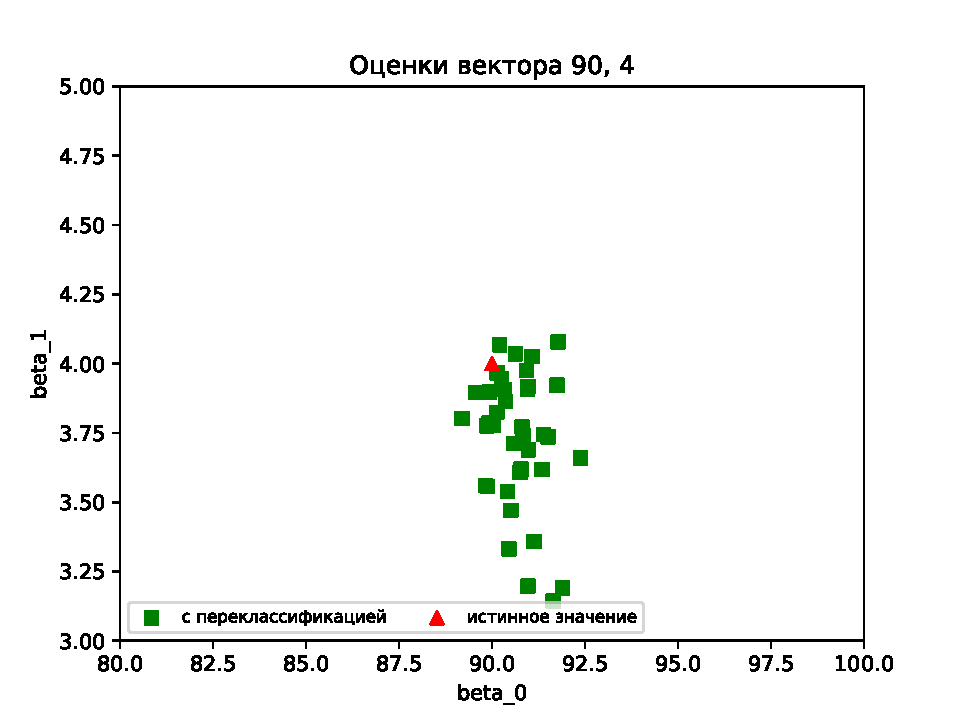
\includegraphics[width=100mm]{pics/plot_90_4_(3).pdf}
    \caption{Вывод графика рассеяния $(\hat{\beta}_0,\hat{\beta}_1)$\label{overflow}}
    \label{pic2}
\end{figure}
\hfill\break

Изобразим на рисунке \ref{pic_3} \textit{100} оценок $\hat{\beta}$ без переклассификации, описанной в пункте \ref{sec4_3}, и с ней:\hfill\break
\begin{figure}[h]
    \centering
    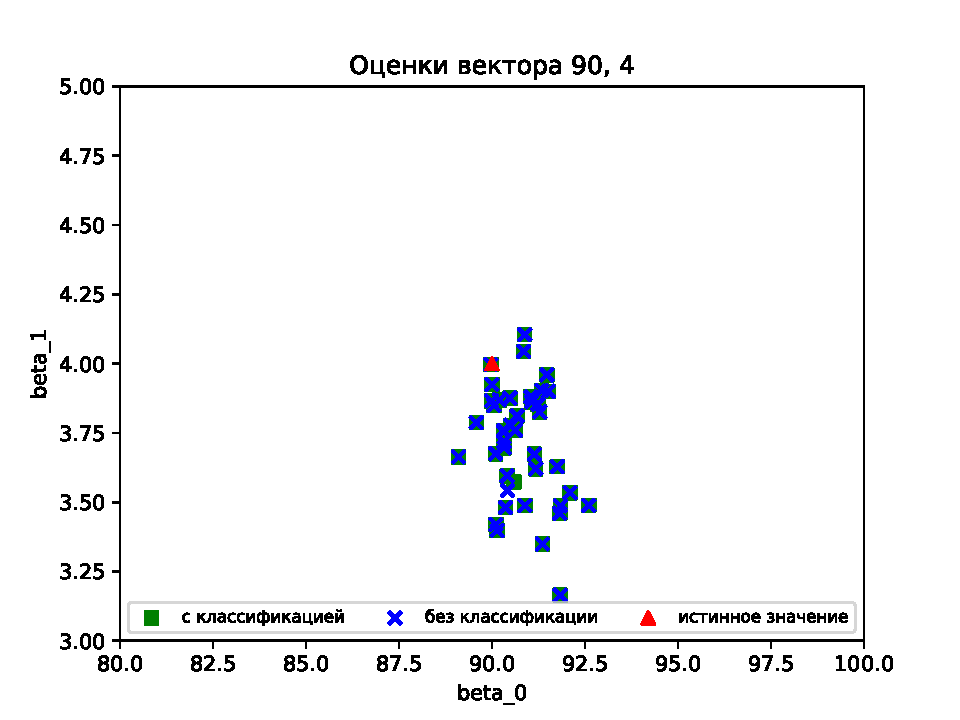
\includegraphics[width=110mm]{pics/plot_90_4_with-without_(3).pdf}
    \caption{Вывод графика рассеяния $(\hat{\beta}_0,\hat{\beta}_1)$\label{overflow}}
    \label{pic_3}
\end{figure}
\break

\newpage
\begin{figure}[ht]
    \centering
    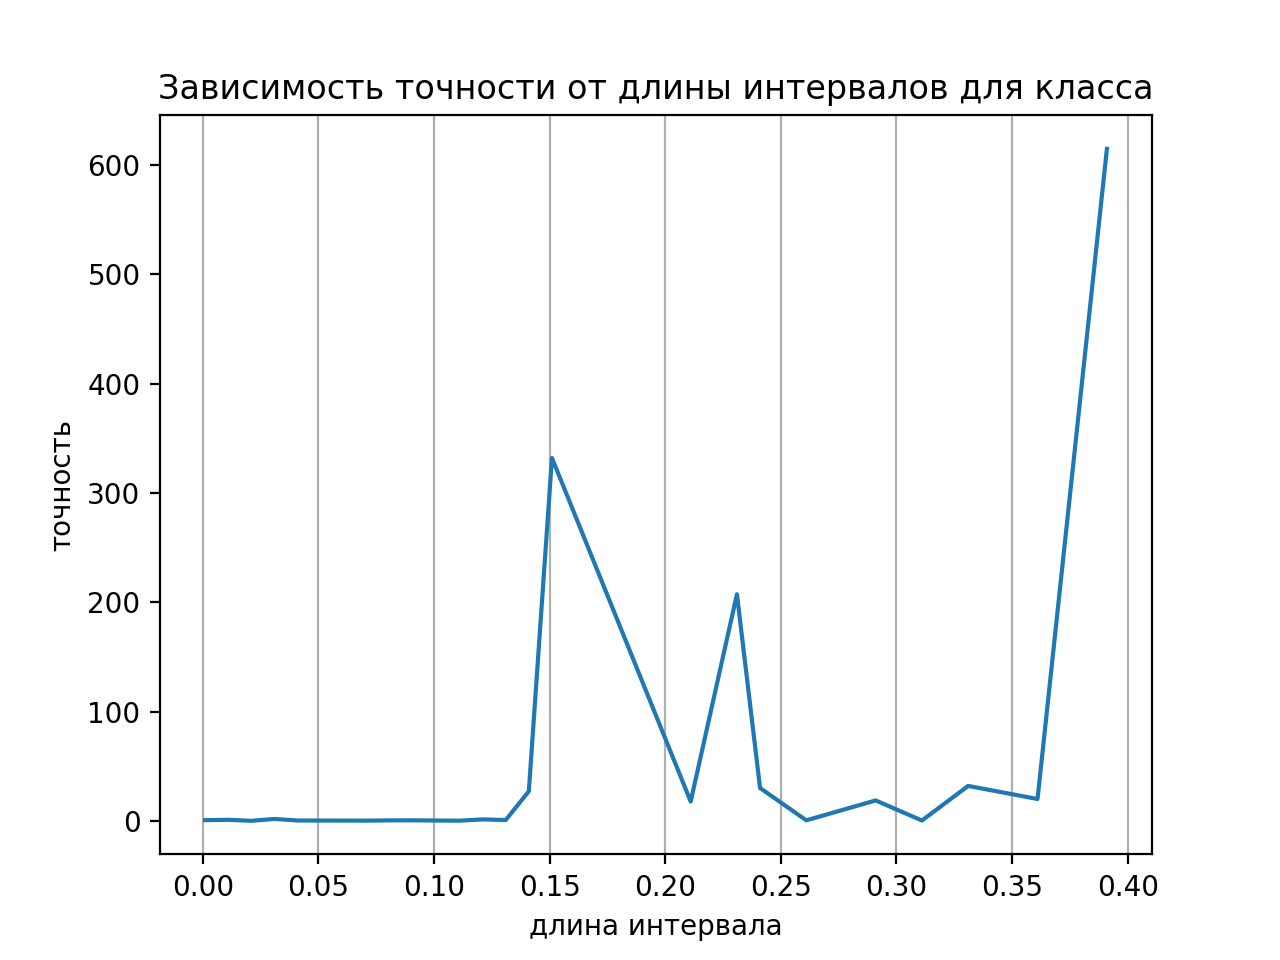
\includegraphics[width=100mm]{pics/plot_90_4_accuracy-length.png}
    \caption{Зависимость точности от длины интервала\label{overflow}}
    \label{pic_4}
\end{figure} 
На рисунках \ref{pic_4}-\ref{pic_5} показана зависимость эмпирической вариации оценок от длины интервалов классификации и объема выборки.
\begin{figure}[hb]
    \centering
    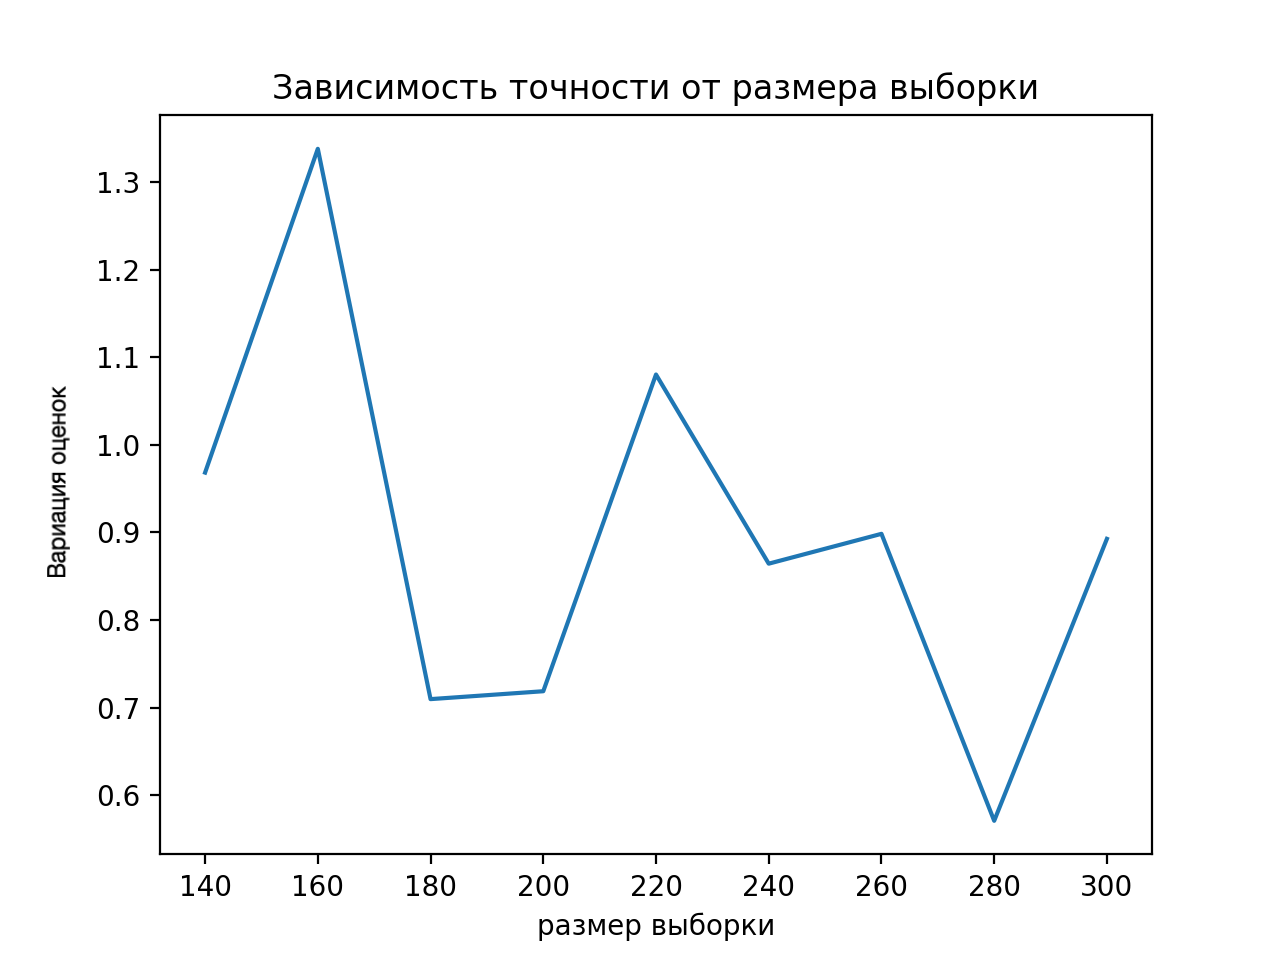
\includegraphics[width=100mm]{pics/plot_90_4_accuracy-samplesize.png}
    \caption{Зависимость точности от размера выборки\label{overflow}}
    \label{pic_5}
\end{figure}
\newpage
\begin{figure}[h]
    \centering
    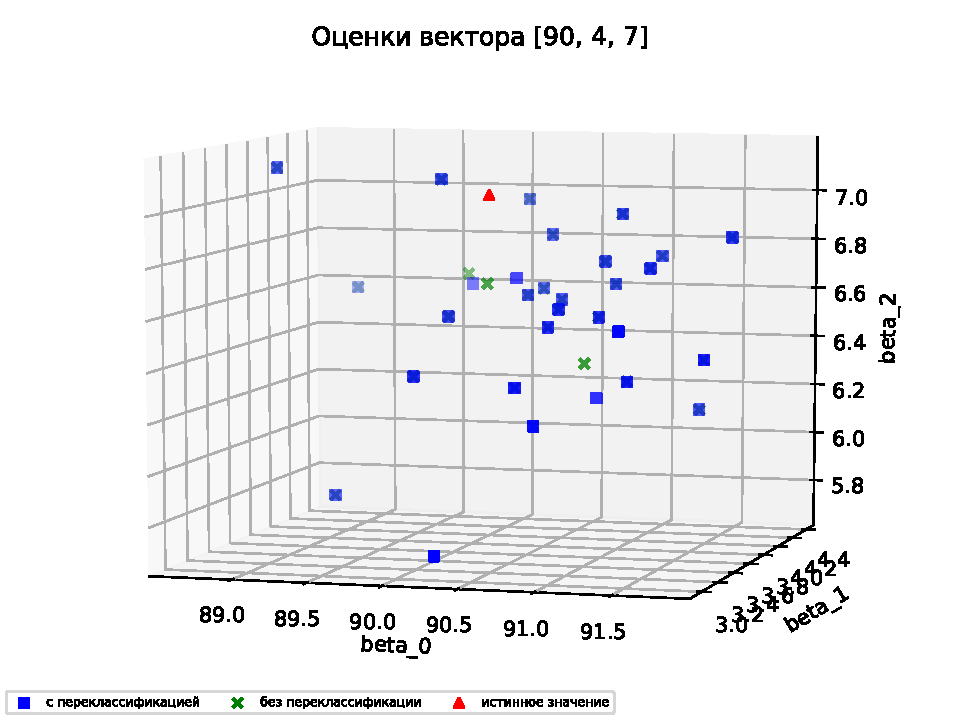
\includegraphics[width=100mm]{pics/plot_90_4_7_(4).pdf}
    \caption{Вывод графика рассеяния $(\hat{\beta}_0,\hat{\beta}_1, \hat{\beta}_2)$\label{overflow}}
    % \label{pic_3}
\end{figure}

Из представленных рисунков можем сделать вывод, что точность увеличивается при увеличении выборки и падает при уменьшении
точности классифицирования. Это не опровергает возможную состоятельность оценок.\hfill\break
\newpage

\begin{center}
    \section*{Заключение}
\end{center}
\phantomsection
\addcontentsline{toc}{section}{Заключение}
В ходе выполнения курсового проекта были получены следующие результаты:
\begin{itemize}
    \item рассмотрена математическая модель линеейной регрессии с выбросами при наличии группирования наблюдений;
    \item описаны основные методы оценивания параметров линейной регрессии при наличии выбросов: оценки МНК, М-оценки;
    \item построены оценки параметров линейной регрессии при наличии группирования наблюдений по методу максимального правдоподобия;
    \item проведены компьютерные эксперименты в которых построенные оценки применялись к модельным данным;
    \item результаты экспериментов показали, что построенные оценки могут быть состоятельными.
\end{itemize}


\newpage
% \section{Список литературы}
% \printbibliography
\begin{thebibliography}{8}
    \bibitem{Huber}
    Хьюбер Дж П.~
    \textit{Робастность в статистике:пер. с англ.} --
    М.:Мир, 1984.-304 с.

    \bibitem{Kharin}
    Харин Ю.С., Зуев Н.М.,
    Жук Е.Е.~
    \textit{Теория вероятностей, математическая и прикладная статистика: учебник} --
    Минск: БГУ, 2011.-463 с.

    

    \bibitem{OLSforGrouping}
    Е. С Агеева, чл.-корр. НАН Беларуси Ю.С. Харин~
    \textit{Состоятельность оценки максимального правдопобия параметров множественной регрессии по классифицированным наблюдениям}

    \bibitem{RobustRegression}
    John Fox, Sanford Weisberg~
    \textit{Robust Regression} --
    October 8, 2013

    \bibitem{RobustPolynomialEstimation}
    А.В. Омельченко~
    \textit{Робастное оценивание параметров полиномиальной регрессии второго порядка} --
    Харьковский национальный университет радиоэлектроники, Украина, 2009

    \bibitem{ComparisonRobust}
    \"{O}zlem G\"{u}r\"{u}nl\"{u} Alma~
    \textit{Comparison of Robust Regression Methods
    in Linear Regression} -- 
    Int. J. Contemp. Math. Sciences, Vol. 6, 2011, no. 9, 409 - 421 с.

    \bibitem{Winitzki}
    Sergei Winitzki~
    \textit{A handy approximation for the error function and its inverse.}

    \bibitem{NumericalMethods}
    Мандрик П.А., Репников В.И., Фалейчик Б.В.,
    \textit{Численные методы} [Электронный ресурс].
\end{thebibliography}
\addcontentsline{toc}{section}{Список Литературы}

\newpage


\section*{Приложение}
\phantomsection
\addcontentsline{toc}{section}{Приложение}
\subsection*{Листинг некоторых методов}
Метод секущих:
\begin{Verbatim}[fontsize=\scriptsize]
def fit_intercept(self, beta_hat=None, beta_hat_next=None):
    if beta_hat is None:
        beta_hat = np.matrix(np.zeros(self.exogen[0].size)).T

    if beta_hat_next is None:
        beta_hat_next = np.matrix(np.ones(self.exogen[0].size)).T

    iteration_counter = 0
    while np.linalg.norm(beta_hat - beta_hat_next) > Defines.METHOD_ACCURACY:
        if self._shared_stop_event.is_set():
            raise StopIteration("fit: got stop event")
        if iteration_counter < Defines.COUNT_LIMIT_OPERATIONS:
            iteration_counter += 1
            dlikelihood_f_for_beta_hat_next = self.full_cl_recl_dlikelihood_f(beta_hat_next)
            delta_beta = np.matrix(np.zeros(self.exogen[0].size)).T

            dlikelihood_derivative_approximation = np.zeros((self.exogen[0].size,
             self.exogen[0].size))

            for i in range(self.exogen[0].size):
                temp_beta = copy.deepcopy(beta_hat_next)
                temp_beta[i] = beta_hat[i]
                dlikelihood_derivative_approximation[i] = ((self.full_cl_recl_dlikelihood_f(
                    beta_hat_next) - self.full_cl_recl_dlikelihood_f(temp_beta)) / (beta_hat_next[i] - beta_hat[i])).A1

            delta_beta = (- np.matrix(dlikelihood_f_for_beta_hat_next)[0] * np.linalg.inv(
                dlikelihood_derivative_approximation))
            beta_hat = beta_hat_next
            beta_hat_next = beta_hat_next + delta_beta.T
        else:
            raise StopIteration("fit: fit_intercept has achieved iteration limit")

    return beta_hat_next
\end{Verbatim}
Решение методом секущих:
\begin{Verbatim}[fontsize=\scriptsize]
def fit(self):
    print("")
    self.classify()
    self.reclassify(Defines.RECLASSIFICATION_LEVEL)

    print("fit: fitting.....")

    t_beta_hat = np.matrix([80.0, 0.0]).T
    t_beta_hat_next = np.matrix([100.0, 10.0]).T
    right_bound_indent = Defines.right_bound_fit_indent(self.exogen[0].size)
    loop_indentantion_value = Defines.LEFT_BOUND_EVERY_VAR_INDENT
    loop_end_bound = Defines.fit_loop_stop_value(self.exogen[0].size)

    beta_hats_left_bound = Defines.left_bound_fit_init(self.exogen[0].size)

    def recursive_beta_generator(index, previous_step_beta):
        assert (index <= self.exogen[0].size)

        beta_next = np.matrix.copy(previous_step_beta)

        while ((beta_next + right_bound_indent) < loop_end_bound).all():
            if index == self.exogen[0].size:
                yield beta_next
                break

            beta_next[index] += loop_indentantion_value

            next_index_generator = recursive_beta_generator(index + 1, beta_next)
            for item in next_index_generator:
                yield item

    fit_intercept_results = []

    def fit_intercept_and_add_to_results(beta_hat_one, beta_hat_two):
        t_result = self.fit_intercept(beta_hat_one, beta_hat_two)
        if (np.isnan(t_result) == False).all():
            print("fit: added value to list %s" % t_result)
            fit_intercept_results.append(t_result)
        else:
            raise Exception("fit: got nan")

    created_threads = []
    for beta_left in recursive_beta_generator(0, beta_hats_left_bound):
        beta_right = beta_left + right_bound_indent
        calculus_thread = Thread(target=fit_intercept_and_add_to_results, args=(np.matrix.copy(beta_left),
                                                                                np.matrix.copy(
                                                                                    beta_right)))
        created_threads.append(calculus_thread)
        calculus_thread.start()

    for thread in created_threads:
        thread.join(timeout=Defines.THREAD_JOIN_TIMEOUT)

    maximum_likelihood_res = None
    result_to_return = np.matrix([None for _ in range(self.exogen[0].size)]).T

    print("fit: possible betas: ")
    print(fit_intercept_results)

    initial_left_bound = Defines.left_bound_fit_init(self.exogen[0].size)
    initial_right_bound = loop_end_bound

    self._shared_stop_event.set()

    for result in fit_intercept_results:
        if (result < initial_left_bound).any():
            continue

        if (result > initial_right_bound).any():
            continue

        t_likelihood_res = self.full_cl_recl_likelihood_f(result)
        # print(t_likelihood_res)
        if maximum_likelihood_res is None:
            maximum_likelihood_res = t_likelihood_res
            result_to_return = result

        if maximum_likelihood_res < t_likelihood_res:
            maximum_likelihood_res = t_likelihood_res
            result_to_return = result

    return result_to_return
\end{Verbatim}
\newpage
\end{document}